\documentclass{article}
\usepackage[utf8]{inputenc}

\title{IF670 - Matemática Discreta para Computação}
\author{Ana Sofia de Oliveira Silva Lima (asosl)}
\date{Setembro 2022}

\usepackage{natbib}
\usepackage{graphicx}

\begin{document}

\maketitle

\section{Introdução} 
    \paragraph{}A cadeira de Matemática Discreta (para Computação), mais conhecida como MD, faz parte dos componentes do 1° período dos cursos do CIn-UFPE. Essa matéria, ministrada pela professora Anjolina Grisi de Oliveira, consiste num curso básico de matemática, necessário para a criação de diversos algoritmos.
    
\section{Relevância}
    \paragraph{}A Matemática Discreta estuda estruturas finitas e objetos separados e desconexos (ao contrário da matemática contínua). Além de desenvolver a maturidade matemática, seu estudo é de grande importância na área computacional, uma vez que pode-se considerar um elemento computacional é um sistema discreto finito. \cite{book1}
    \paragraph{}Esse estudo pode ser usado para a Modelagem Matemática, que "constitui-se em um conjunto de procedimentos cujo objetivo é estabelecer um paralelo para tentar explicar, matematicamente, os fenômenos presentes no cotidiano do ser humano, ajudando-o a fazer predições e a tomar decisões" \cite{paper1}. Dessa forma, pode ser aplicado e ajuda a desenvolver diversos ramos da computação, tais quais: projeto de algoritmos, robótica, rede de computadores, circuitos integrados, inteligência artificial e etc. \cite{paper2}
    
    \begin{figure}
        \centering
        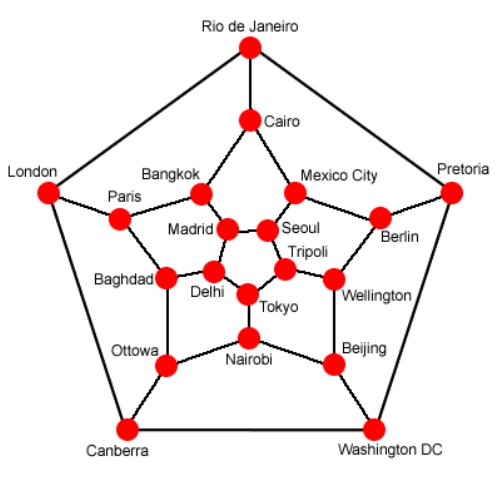
\includegraphics[width=5cm, height=5cm]{grafos.png}
        \caption{A imagem mostra um grafo, objeto de estudo da Matemática Discreta, que pode ser usado amplamente na computação, como em \textit{machine learning} \cite{fig1}.}
        \label{Figura 1}
    \end{figure}
    
\section{Relação com as outras matérias}
	\paragraph{}Visto que é componente obrigatório do primeiro período do curso, não há pré-requisitos para essa cadeira, poŕem ela é necessária para outras matérias do segundo período, IF673 - LÓGICA PARA COMPUTAÇÃO; e do quarto período (indiretamente, já que estas tem como pré-requisito a IF673), IF689 - INFORMÁTICA TEÓRICA, IF682 - ENGENHARIA DE SOFTWARE E SISTEMAS e IF684 - SISTEMAS INTELIGENTES. A partir dessas cadeiras do segundo e quarto período, existem muitas outras eletivas que dependem dos conteúdos ministrados em Matemática Discreta para Computação. \cite{site1}

\section{Organização}
	\paragraph{}A cadeira é dividida em duas unidades e, na modalidade presencial, há uma avaliação e um ponto extra (separado em uma ou duas mini-provas - feitas e aplicadas pelos monitores) para cada uma dessas unidades. Os assuntos são:
	\paragraph{1ª unidade:}Provas e proposições, noções básicas sobre conjuntos, noções básicas sobre funções e relações, sequências, cardinalidade e enumerabilidade, racionais, crescimento de função, métodos de prova e indução matemática, definições recursivas, teorema binomial, triângulo de Pascal, O Princípio da Casa de Pombo, números primos e divisibilidade, Algoritmo de Euclides, aritmética modular, Teorema Chinês do Resto, o pequeno teorema de Fermat e teste de primalidade.

	\paragraph{2ª unidade:}Relações, fechos de uma relação, relações de equivalência, ordenações parciais, ordem lexicográfica, Diagrama de Hasse, reticulados, grafos, planaridade, coloração e árvores.


\bibliographystyle{plain}
\bibliography{ref}

\end{document}